\section{Identification d'un grillage}
Si un grillage est un ensemble de lignes, il possède d'autres propriétés particulières qui aident à sa reconnaissance. Sa périodicité spatiale ainsi que l'angle formé entre les duex directions du grillage en font partie. Nous nous sommes donc tout d'abord intéressés à la reconnaissance de ces éléments dans la transformée de Hough. 

\subsection{Reconnaissance du grillage dans la transformée de Hough}
\subsubsection{Hypothèses}
Tout d'abord on peut supposer que les deux directions du grillage sont approximativemnt perpendiculaires (à $90\text{°} \pm 30\text{°}$). Deux paquets de piques doivent donc être visibles avec cet écart d'angle sur la transformée de Hough.

En outre supposons le grillage pris de face comme en figure  \ref{houghlines}, ses lignes  détectées auparavant possèdent alors la particularité d'avoir toutes le même angle $\theta$ et de varier périodiquement en $\rho$ comme on le voit sur sa transformée de Hough en figure \ref{houghlines}. Si le grillage est observé de biais les angles des lignes varient comme on peut le voir sur l'image d'exemple \ref{houghlines}. Leur représentation dans la transformée de Hough en figure \ref{houghlines} n'est plus une droite verticale ni même une droite et les valeurs de $\rho$ correspondantes ne sont plus périodiques.

\begin{figure}[h]
\begin{center}
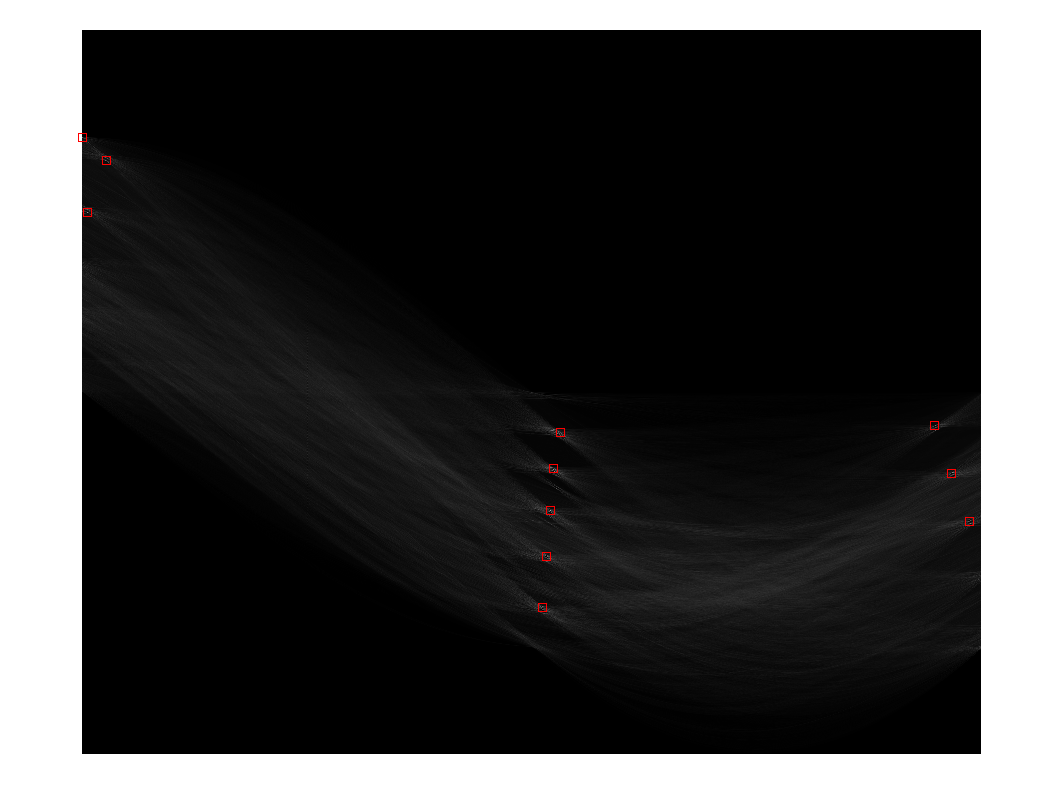
\includegraphics[scale=0.23]{fig/centrageavt.png}
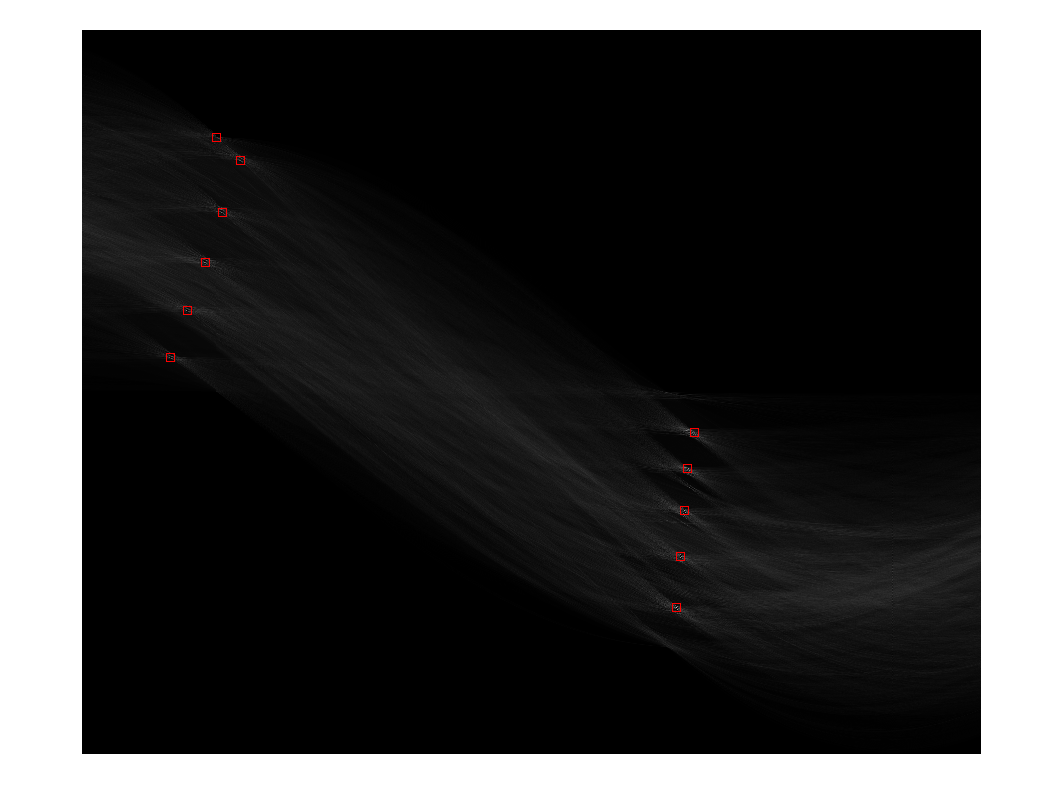
\includegraphics[scale=0.23]{fig/centrageapres.png}
\caption{\label{centrage} Centrage de la transformée de Hough, à gauche la transformée de Hough non centrée, à droite la transformée de Hough centrée.\\ La ligne coupée dans la transformée de Hough ne l'est plus après centrage et peut être détectée.}
\end{center}
\end{figure}

Nous supposerons que le grillage n'est pas pris trop de biais comme présenté avant, on peut alors espérer détecter des lignes dans Hough, ou plus précisément deux lignes dont les abscisses (l'angle moyen des lignes détectées dans l'image) sont séparées d'environ 90 \degre.

\subsubsection{RANSAC dans la transformée de Hough}
Tout d'abord nous centrons la transformée de Hough de manière à ce que les lignes que l'on désirait y détecter ne soient pas coupées. En effet la transformée de Hough détecte les lignes dans l'image dont l'angle est compris entre -90° et 90°. Si le grillage comprend une direction horizontale déformée par la prise de vue, les lignes détectées selon cette direction peuvent avoir des angles à la fois légèrement supérieurs à -90° et légèrement inférieurs à 90°. Or elles forment ensemble un potentiel grillage que l'on aimerait détecter dans la transformée de Hough.

Concrètement nous réalisons une permutation de la transformée de Hough selon l'axe des abscisses jusqu'à ce que la zone coupée (au niveaux de  l'abscisse 0 et de l'abscisse maximale) contienne un minimum de piques de la transformée de Hough. Ce centrage est illustré en figure \ref{centrage}.

\begin{figure}[h]
\begin{center}
\begin{tabular}{cc}
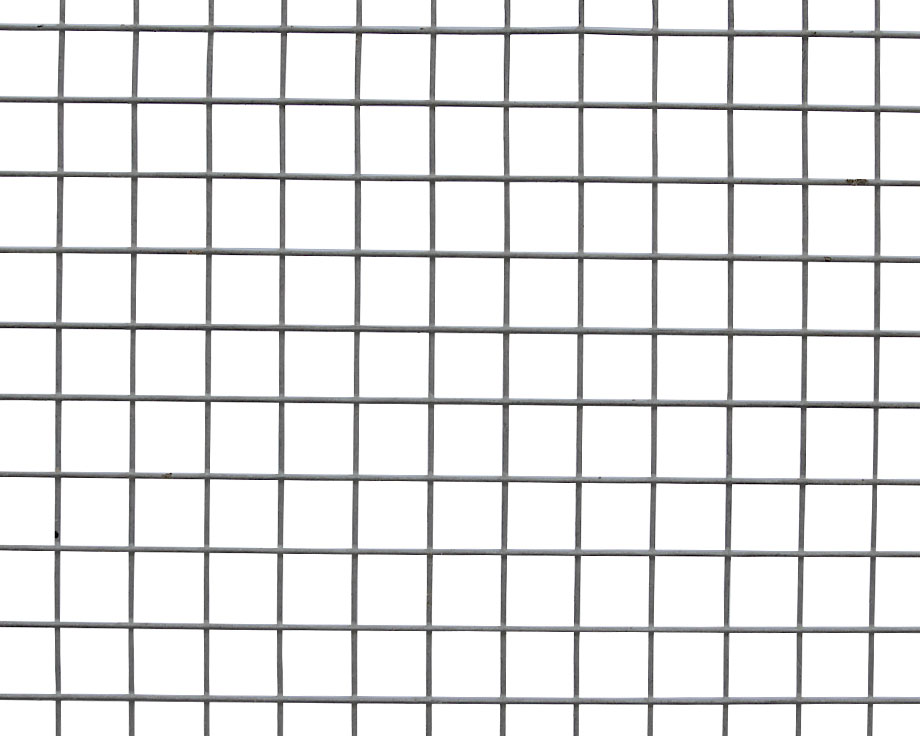
\includegraphics[scale=0.18]{fig/grillage.jpg} &
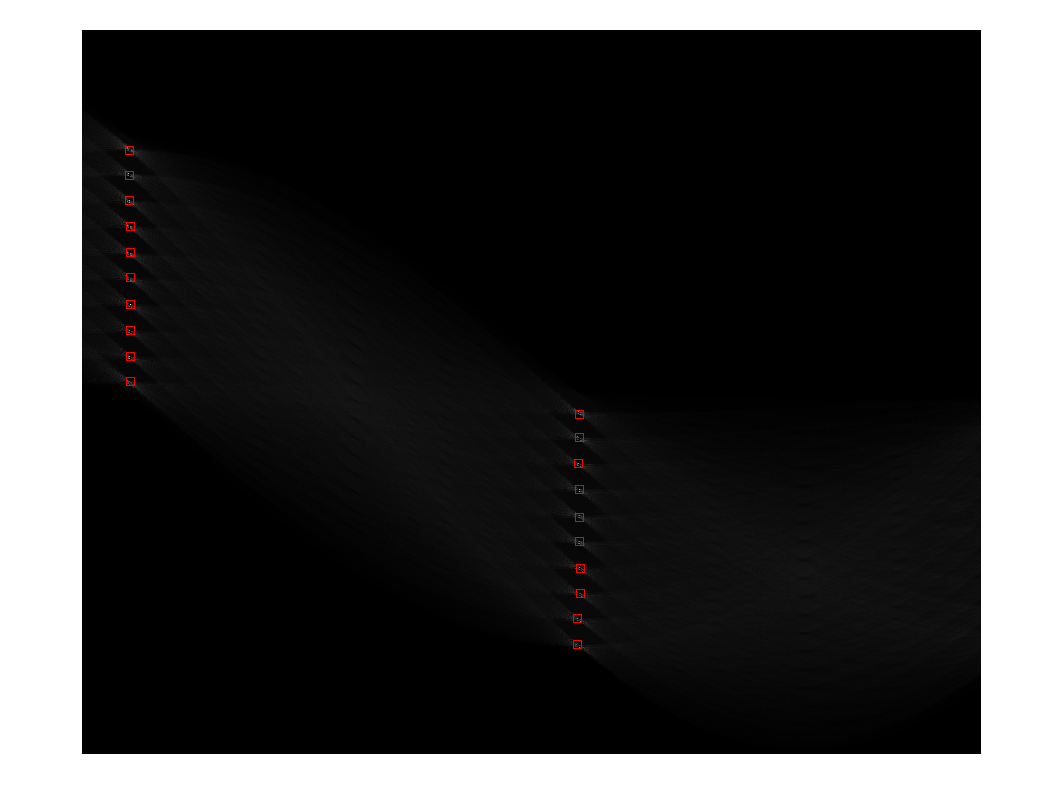
\includegraphics[scale=0.2]{fig/grillagehough.png}
\\
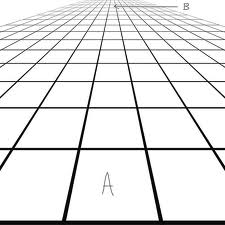
\includegraphics[scale=0.4]{fig/perspective.jpg}
& 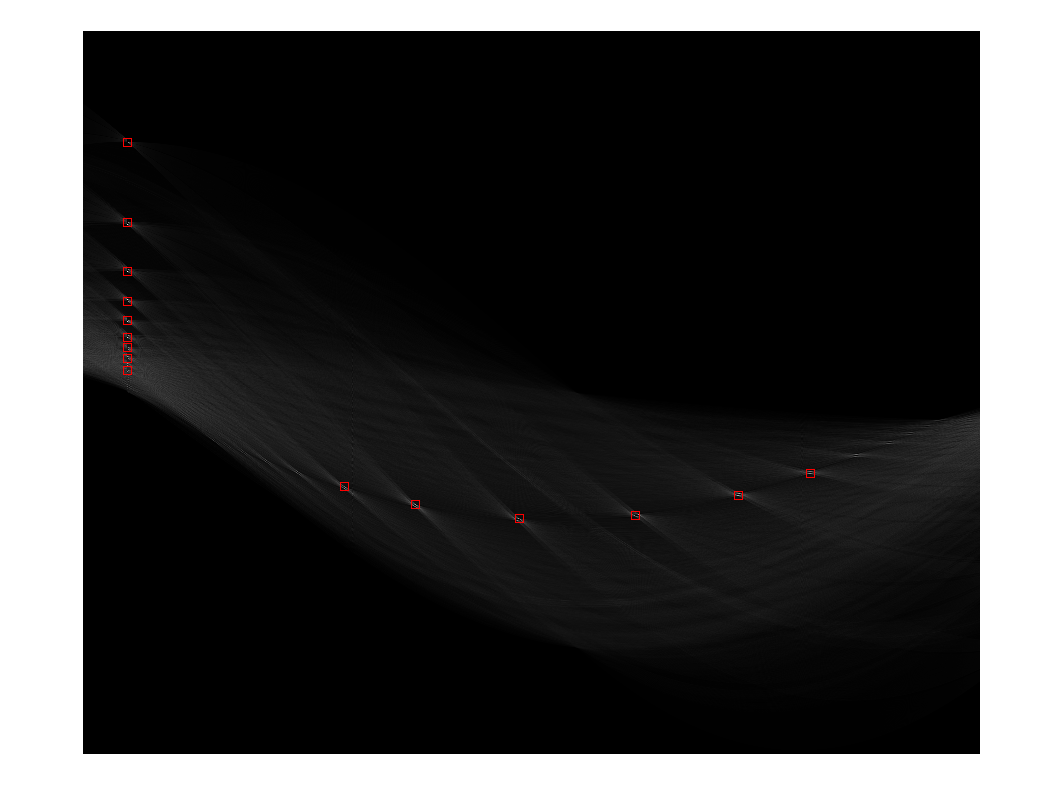
\includegraphics[scale=0.2]{fig/perspectivehough.png}
\end{tabular}
\caption{\label{houghlines} Illustration de l'impact de la perspective sur les piques troués dans la transformée de Hough. \\A gauche les images, à droite leurs transformée de Hough respectives. }
\end{center}
\end{figure}

Nous avons observé dans la transformée de Hough des artéfacts au niveau en abscisse des angles $\theta=-90\text{°},-45\text{°},45\text{°},90\text{°}$. Il s'agit en quelque sorte d'un décalage de la transformée de Hough à ces angles menant à la détection de faux piques à leurs niveaux. Nous éliminons donc tous les piques pouvant être détectés à ces abscisses avant de procéder à la suite.
\\

Nous avons tout d'abord tenté de reconnaître des lignes dans la transformée de Hough par une seconde transformée de Hough sur la transformé de Hough. Cependant cette méthode était trop rigide car elle ne permettait pas de reconnaître le grillage si celui-ci était pris trop en biais et ne s'illustrait donc pas tout à fait comme une droite sur l'image.
\\

Nous avons donc affiné notre méthode en essayant de reconnaître ces droites à l'aide d'un algorithme RANSAC appliqué sur des fenêtres de la transformée de Hough. RANSAC a en effet l'avantage d'offrir plus de souplesse qu'une transformée de Hough sur la transformée de Hough tout en gardant l'idée de détecter des lignes et non de chercher un simple agglomérat de piques dans la transformée de Hough. Cette amélioration est illustrée en figure \ref{houglines}

\begin{figure}[h]
\begin{center}
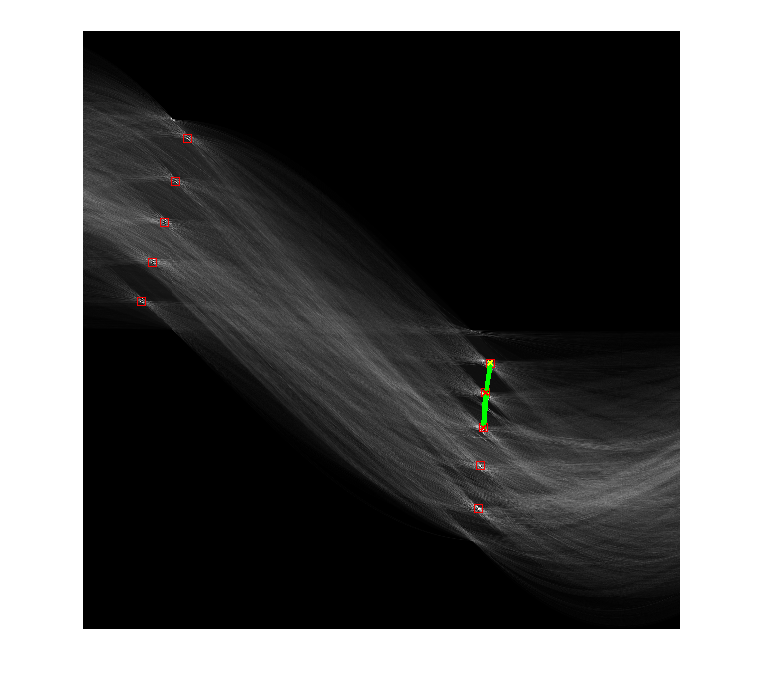
\includegraphics[scale=0.238]{fig/houghlineshough.png}
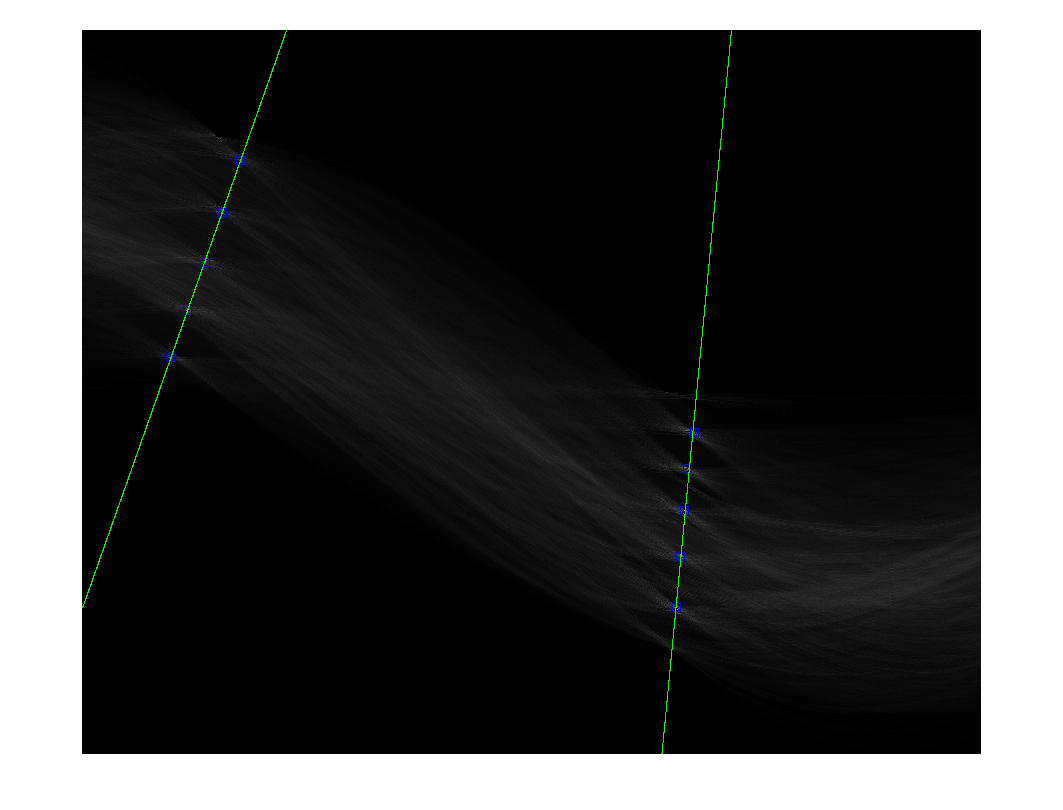
\includegraphics[scale=0.2]{fig/houghlinesRANSAC.png}
\caption{\label{houghlines}Détections de droites dans la transformée de Hough grâce à gauche à une seconde transformée de Hough et à droite avec RANSAC \\
On observe que les points ne sont pas tout à fait alignés pour qu'une seconde transformée de Hough les détecte alors qu'un RANSAC y parvient mieux.}
\end{center}
\end{figure}

Concrètement nous prenons deux larges fenêtres dans la transformée de Hough dont la largeur horizontale est de 30° (couvrant ainsi les lignes de l'image dont les directions sont semblables à 30° près) et la largeur verticale est celle de la transformée de Hough. Ces fenêtres sont espacées de 90° illustrant la détection des deux directions du grillage et non de simples lignes parallèles dans l'image. 

Dans chacune de ces fenêtres nous utilisons un algorithme RANSAC afin de détecter les lignes dans la transformée de Hough qui s'y trouvent. Nous utilisons RANSAC pour éviter de prendre en compte des piques de la transformée de Hough qui n'ont rien à voir avec le grillage dans la fenêtre prise en compte et qui fausseraient la détection de la ligne. 

Nous faisons ensuite glisser cette paire de fenêtres pour couvrir la totalité de la transformée de Hough. Pour chacune des paires de fenêtres nous calculons le nombre de piques se trouvant près de la ligne détectée par RANSAC dans chacune des deux fenêtres. Cela nous donne un premier score. Si la ligne trouvée dans la transformée de Hough est trop horizontale on considère que c'est une erreur et nous donnons un score de 0. Nous choisissons finalement la paire de fenêtres au score maximal. 


Cette étape nous donne ainsi un premier grillage potentiel comme illustré en figure \ref{grillage1} parfois complet dans des cas simples comme celui présenté ici. En prenant de larges fenêtres nous pallions le problème de la prise de vue en biais qui déformerait les directions des lignes du grillage. L'utilisation de RANSAC dans ces larges fenêtres permet ensuite de détecter des lignes sans être dérangé par des piques ne décrivant pas des lignes du grillage. 

\begin{figure}[h]
\begin{center}
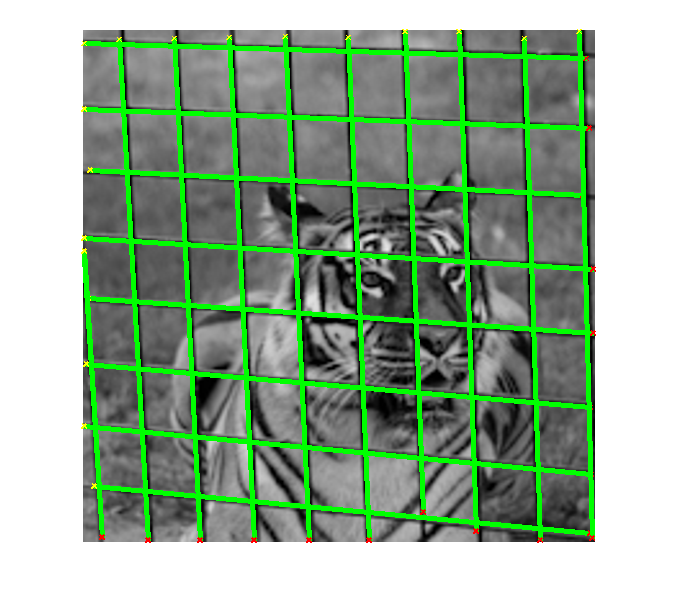
\includegraphics[scale=0.4]{fig/grillage1.png}
\caption{\label{grillage1}Exemple de grillage obtenu avec la première méthode.}
\end{center}
\end{figure}

\subsection{Validation du grillage obtenu}
Une fois un premier grillage trouvé nous aurions aimé le valider grâce à l'image en utilisant des descripteurs différents de la détection de contours par méthode de Canny.
\\

Une première solution était de vérifier s'il existait une périodicité de couleur au niveau du grillage détecté. En effet si on se place selon une direction du grillage et en dehors de ce dernier, la seconde direction devrait apparaître périodiquement par ses lignes qu'on reconnaît à leur couleur

Cependant cette méthode peut être mise à mal pour deux raisons. Tout d'abord il faudrait que le grillage ait une couleur relativement unie, or l'éclairage de la photo met en danger cette hypothèse. En outre, comme dit précédemment, la prise de vue de la photo peut faire perdre la périodicité spatiale du grillage rendant cette méthode caduque. C'est pourquoi nous n'avons finalement pas mis en place cette méthode.
\\

Une deuxième solution pouvait être d'utiliser des transformées morphologiques. Nous avons notamment pensé à réalisé un gradient morphologique avec pour élément structurant un segment de direction l'une de celles du grillage.
\\

Nous n'avons finalement pas validé les grillages obtenus car ils étaient dans une grande majorité des cas bons dès la première approche. Ceci est notamment dû à la qualité de notre premier détecteur et donc du choix de la résolution adoptée pour l'image.


\subsection{Raffinement du grillage}
Le premier grillage obtenu est le plus souvent incomplet : les deux directions du grillage sont connues ainsi qu'un certain nombre de barreaux mais pas tous. Nous avons donc essayé plusieurs méthodes pour raffiner ce premier grillage.


\subsubsection{Utilisation des couleurs de l'image}
Connaissant une partie des barreaux nous avons essayé de trouver la couleur du grillage. Pour cela nous avons sélectionner les pixels de l'image situés près des lignes que nous avions trouvé puis nous avons réalisé un K-means couleur sur l'ensemble de ces pixels en espérant que la classe majoritaire du K-means corresponde ainsi à la couleur du grillage.

Malheureusement la classe majoritaire ne correspond pas à la couleur du grillage. Cela peut s'expliquer notamment par le fait que nous détectons les contours du grillage et les lignes ainsi trouvées n'étant pas centrées sur le grillage, les pixels sélectionnés sont souvent hors du grillage. Pour mieux le comprendre nous avons affichés les valeurs des couleurs dans l'espace RGB de ces pixels en figure \ref{Kmeans} : aucun paquet précis ne semble s'y former.

\begin{figure}[h]
\begin{center}
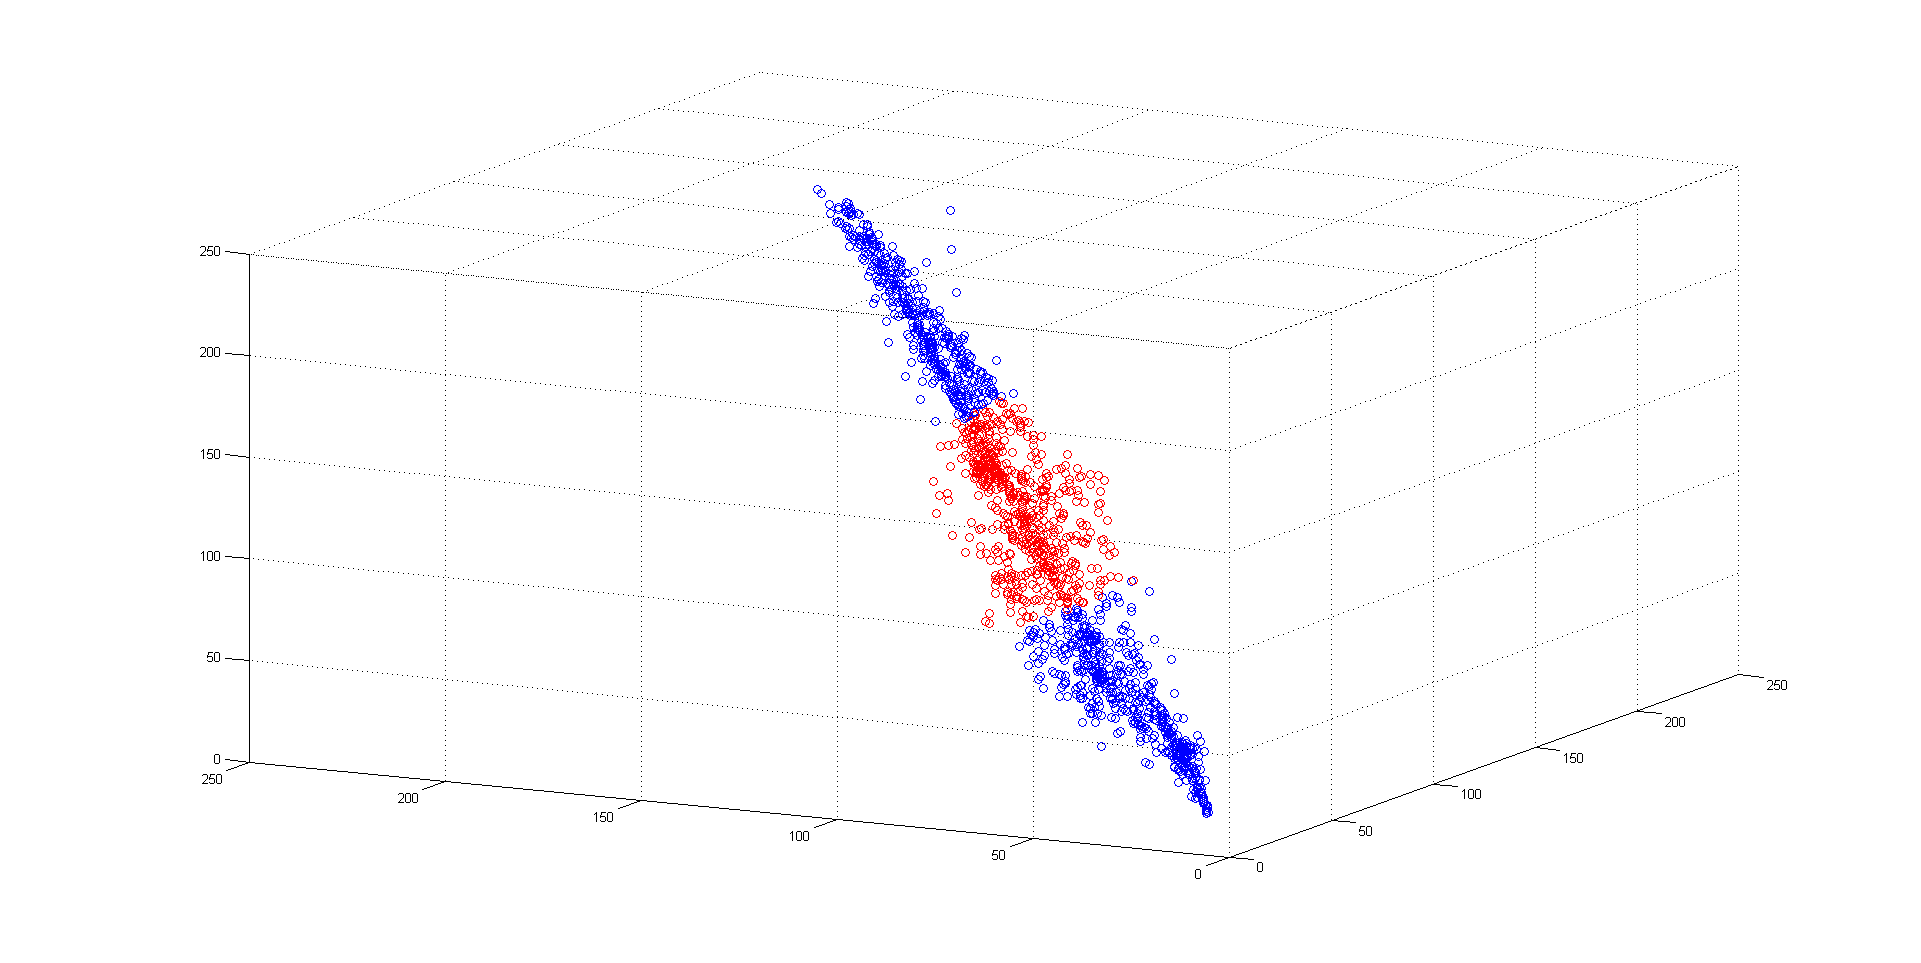
\includegraphics[scale=0.2]{fig/Kmeans.png}
\caption{\label{Kmeans}Couleurs des pixels proches des lignes détectées dans l'espace RGB. En rouge le paquet le plus gros trouvé.}
\end{center}
\end{figure}

\subsection{Utilisation de la périodicité du grillage dans la transformée de Hough}
Comme dit précédemment, en supposant la photo prise relativement face au grillage l'écart en les piques d'une direction du grillage est sensiblement toujours le même : la périodicité du grillage se retrouve ainsi dans la transformée de Hough.

Pour chaque ligne dans la transformée de Hough trouvée précédemment nous calculons l'écart entre les pics sur la ligne. Nous calculons ensuite l'écart moyen en évitant de prendre en compte des valeurs aberrantes à l'aide d'un RANSAC 1D. En effet n'ayant pas tous les barreaux nous espérons en avoir suffisamment pour mettre en évidence la période, si entre deux barreaux, 5 n'ont pas été trouvé l'écart entre leurs piques sur la transformée de Fourier ne sera pas pertinent c'est pourquoi nous évitons de le prendre en compte.

Une fois cette période trouvée dans la transformée de Hough, nous prenons un pique de départ. Pour cela nous remontons selon la ligne trouvée sur la transformée de Hough pas à pas, la pas étant égal à la période trouvée, ceci jusqu'à être en dehors de la transformée de Hough. Nous redescendons ensuite selon la ligne selon ce même pas. A chaque pas, nous "zoomons" sur des petites fenêtres centrées en là où devrait se trouver un pique. Si un pique déjà trouvé s'y trouve nous le prenons et nous repartons de sa position sinon nous cherchons le maximum dans cette fenêtre comme pique. En repartant de points déjà trouvés nous évitons de propager l'erreur due à l'approximation de la période. En effet comme on l'a déjà vu avec la grille en perspective, dans le cas de grillages pris en biais les piques ne sont pas séparés tout à fait régulièrement.

Cette méthode permet de trouver de nombreux nouveaux piques. Cependant il reste parfois quelques rares barreaux non détectés. Pour cela nous pourrions repasser sur l'image, calculer l'écart successif entre les barreaux selon chacune des directions du grillage et chaque fois que l'écart double approximer l'existence d'un barreau au milieu de cet écart. Nous n'avons pas mis en place ce dernier raffinement car il est possible que jouer sur les informations recueillies à différentes résolutions ou utiliser plus intelligemment les transformées morphologiques donnent un résultat plus précis. En  outre dans de nombreux cas ce raffinement suffit.

Nous présentons en figure \ref{grillage2} le résultat avant et après raffinement selon la méthode proposée ici. On constate que de nombreux nouveaux barreaux ont été trouvé mais qu'il en manque encore et que certains ont été ajouté.

\begin{figure}[h]
\begin{center}
\begin{tabular}{cc}
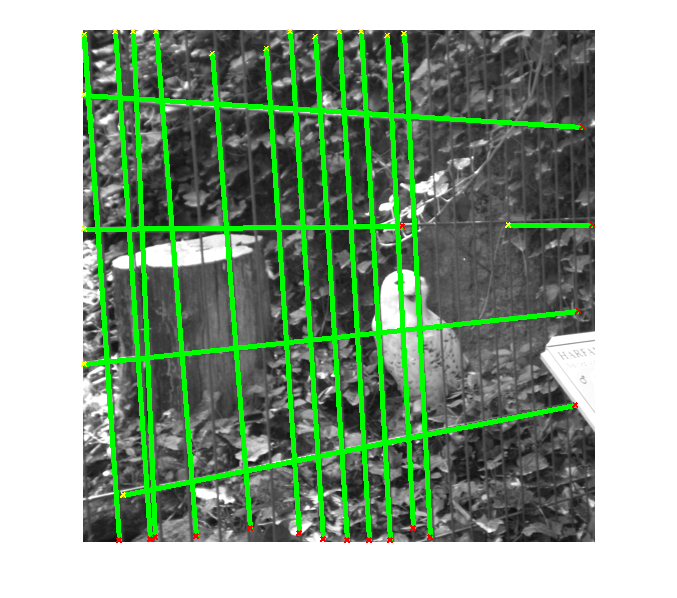
\includegraphics[scale=0.3]{fig/grillagesansraf.png}
& 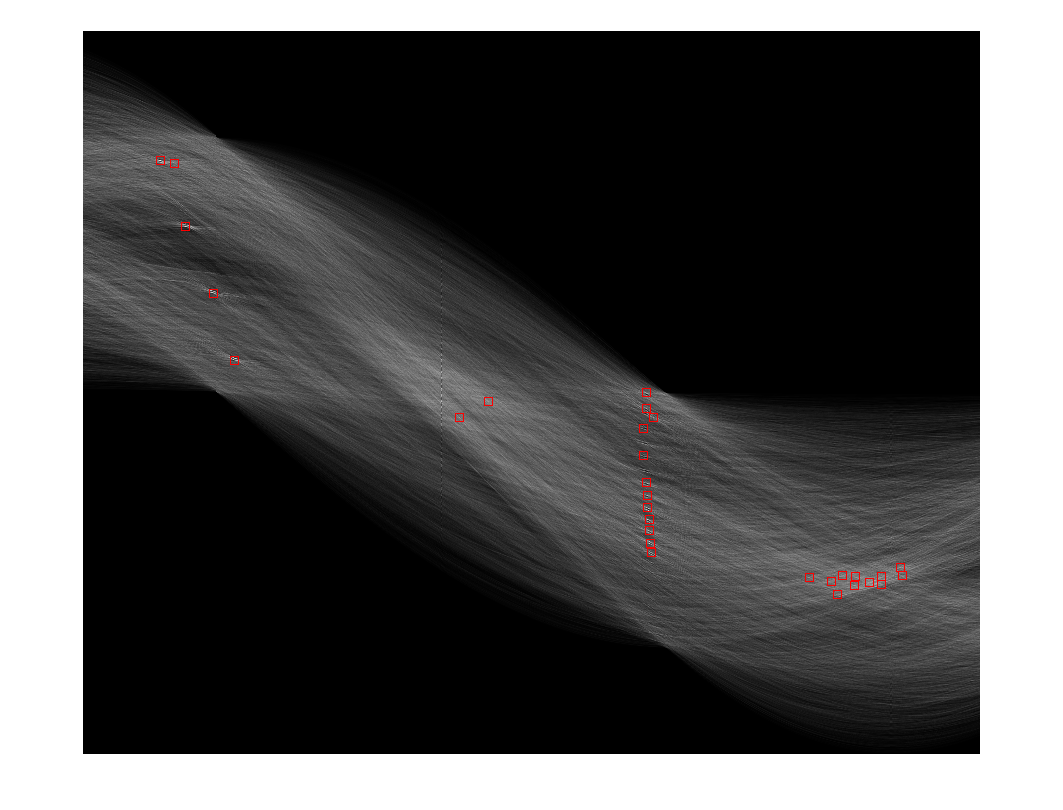
\includegraphics[scale=0.2]{fig/houghsansraf.png} \\
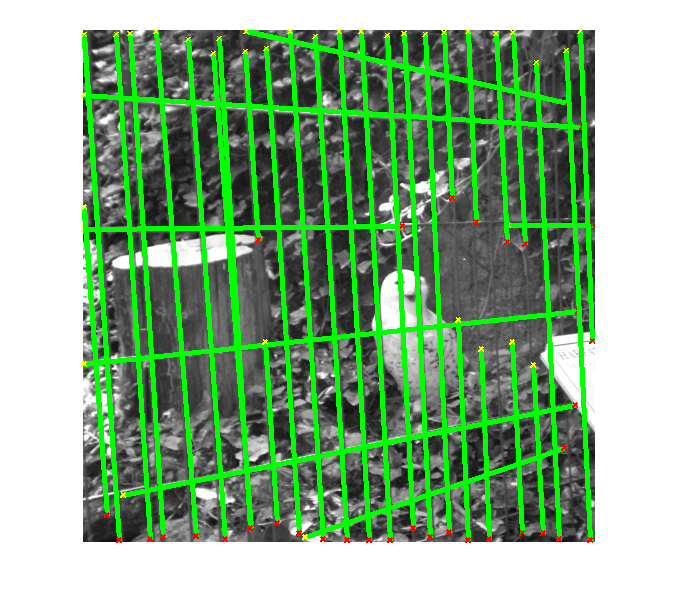
\includegraphics[scale=0.3]{fig/grillageavecraf.png}
& 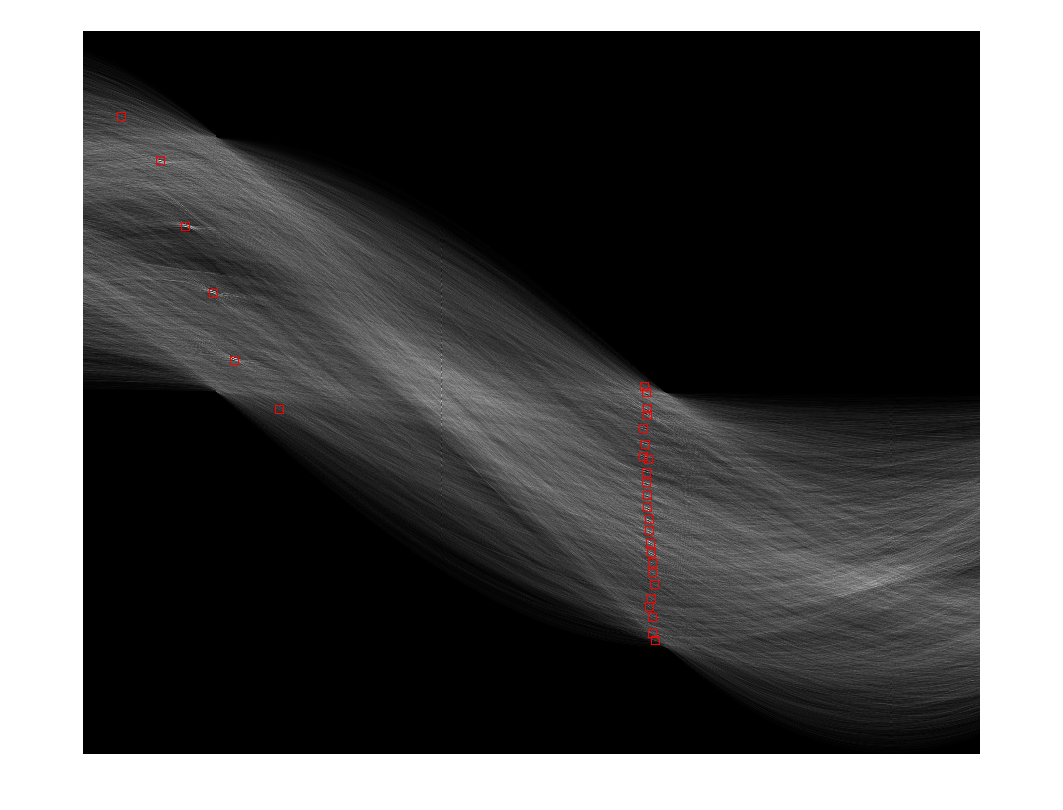
\includegraphics[scale=0.2]{fig/houghavecraf.png}
\end{tabular}

\caption{\label{grillage2} Raffinement du grillage en utilisant la périodicité du grillage dans Hough\\
A gauche on observe les images, à droite leurs transformées de Hough et les piques détectés. En haut il s'agit du premier grillage détecté avec la méthode précédente, en bas avec le raffinement.}
\end{center}
\end{figure}




